\cotefile{156-7}
\scanpage{94}
\mspage{93}

J'aimerais prouver le

\uline{\unsure{Théorème}} \textcircled{a} L'application \unsure{précédente} est \unsure{injective}, plus précisément elle induit un \uline{iso. d'ens ordonnés} de $P(\widetilde F)$ sur \deleted{\unsure{le}} un sous-ensemble ordonné de $\Sigma_M$. \textcircled{b} Cette application \deleted{\unsure{est}} commute aux $\operatorname{Sup}$ \margin{facile. $\checkmark$} (tautologiquement) et aux $\operatorname{Inf}$ quelconques. \textcircled{c} On a, pour deux $A,\deleted{\unsure{A}}B\in P(\widetilde F)$, avec $B\subset A$
\[
\deleted{\unsure{S_{B\setminus A}|S_{B\cap A}}=\unsure{S_B}}
\qquad S_{A\setminus B}=S_A\cap C_M(S_B)
\]
\[
\deleted{\unsure{\operatorname{Supp}F}=\unsure{\operatorname{Supp}|S_{\widetilde F}}}
\]
où $C_M$ est l'anti-involution canonique de l'ens. des supports. (\unsure{application cosupport}).

\textcircled{d} \deleted{On a} Si $A$ est une partie \uuline{fermée} de $\widetilde F$ (donc de la forme $\widetilde{\unsure{G|C}}$, où $G\subseteq F$ est une sous-figure de $\unsure{A|\Lambda}$) on a
\[
S_A=\operatorname{Supp}G\overset{\mathrm{def}}=\operatorname{Supp}_{\widehat M}(A)
\]

\uline{NB} En fait, $S_A$ est défini \unsure{sans référence} à la figure ambiante \deleted{\unsure{\(\Phi\)}} $F$, où $\widetilde F=\Phi\subset M$, en termes de l'ens $A\subset M$ formé des multistrates mutuellement compatibles. Donc \unsure{tout} ce formulaire précédent peut se
\scanpage{95}
\mspage{94}

formuler ainsi, en termes d'opérations sur des parties $A,B,A_i$ de $M$, pas néc. fermées, et formées d'objets mutuellement compatibles.

Commençons par d) (\unsure{O.P.S.|Q.P.S.} $A=\widetilde F$)
\[
S_{\widetilde F}\overset{\mathrm{def}}=\operatorname{Supp}\left(\bigcup_{X\in\widetilde F}\unsure{X^\circ|X^0|X^o}\right)=\operatorname{Supp}\deleted{\unsure{X}}F
\]
ce qui revient, par définition des supports, à avoir, pour $\forall Y\in M$
\diagram{\begin{tikzcd}[ampersand replacement=\&,column sep=large,row sep=large]
Y\parallel\deleted{\unsure{X}}F \arrow[r,Leftrightarrow] \arrow[d,Leftrightarrow] \& \forall X\in\widetilde F,\ Y\parallel X^\circ \\
(Y\parallel\widetilde F) \&
\end{tikzcd}}
et cela résulte aussitôt du cor. au lemme 1.

Voyons a) i.e
\[
S_A\subset S_B\quad\Rightarrow\quad A\subset B
\]
Soit donc $X\in A$, on doit prouver $X\in B$, on est ramené à prouver que
\diagram{\begin{tikzcd}[ampersand replacement=\&,column sep=small,row sep=small]
S_{\{X\}} \arrow[d,equal] \& {}\subset S_B\quad\Rightarrow\quad X\in B \\
\operatorname{supp}(X^\circ) \&
\end{tikzcd}}
i.e.

\uline{Lemme \unsure{3|8}} Soient $X\in M$, $B\subset M$, tels que $B\cup\{X\}$ soit admissible (formé d'objets mutuellement admissibles) alors
\[
X^\circ\in S_B\quad\Rightarrow\quad X\in B
\]
% slanted
\margin{\uline{NB} Cela \deleted{\unsure{implique|montre}} comment \unsure{récupérer} $B$ en termes de $S_B$}
Le premier mb \deleted{\unsure{implique}, \unsure{en prenant}} comporte
\[
\forall Z\ \deleted{\unsure{\in M|\in A}}\text{ tel que }Z\parallel\bigcup_{Y\in B}Y^\circ,\quad\text{on a }Z\parallel\deleted{\unsure{Y}}X^\circ
\]
\scanpage{96}
\mspage{95}

donc tout revient à montrer ceci:
\[
X\notin B\quad\Rightarrow\quad\exists Z\in M,\quad Z\parallel\bigcup_{Y\in B}\unsure{Y^\circ|Y^0|Y^o}\quad\text{et}\quad Z\mathrel{\overline{\parallel}}X^\circ
\]
et pour ceci, il suffit de prendre
\[
Z\in X^\circ\qquad\text{(\unsure{Existe} par L1, impliquant }X^\circ\ne\varnothing\text{)}
\]
et appliquer le

\margin{$\big\vert\!\big\vert\!\big\vert$}
\uline{Lemme 4} Soient $X,Y\in M$, $X\unsure{\gtrless|\lessgtr|\asymp}Y$, $X\ne Y$.

Alors $X^\circ\parallel Y^\circ$ (a fortiori, $X^\circ\cap Y^\circ=\varnothing$)

Soient $X'\in X^\circ$, $Y'\in Y^\circ$, il faut prouver $X'\parallel Y'$.
Soit $L=X\cap Y$. Par Ax D, il suffit de prouver $X'_L\parallel Y'_L$. Si $L\leq\partial X,\partial\deleted{\unsure{X}}Y$, \inserted{i.e. $L\ne X,Y$} \deleted{\unsure{et ainsi|et ceci}} on \unsure{aura|a}
\[
X'_L\leq X'_{\partial X}=\varnothing,\quad Y'_L\leq Y'_{\partial X}=\varnothing
\]
donc $X'_L=Y'_L=\varnothing$, OK. Sinon \deleted{\unsure{supposons}} supposons p.ex. $L=\unsure{Y|X}$ i.e. $Y\leq X$. Comme $Y\ne X$, on a $Y'\leq Y\leq\partial X$, et on a $X'\parallel\partial X$ i.e. $X'\parallel Y'$, OK.

Pour prouver b), \deleted{\unsure{comme on a}} pour les $\operatorname{Inf}$ (le \unsure{sachant} pour les $\operatorname{sup}$) on est ramené à prouver la \deleted{\unsure{relation}} compatibilité c) pour les complémentations. \deleted{On a}
\scanpage{97}
\mspage{96}

En fait, le th. est un \deleted{conséquence} \inserted{cas particulier} de l'énoncé formel que voici:

\margin{?}
% slanted
\margin{Faux}
\uline{Lemme} Soit $M$ un ens muni d'une relation sym. antiréflexive $\parallel$, d'où une notion de cosupport, support pour une partie de $M$, et l'ensemble $\overline\Sigma_{\deleted{\unsure{M|A}}}=\overline\Sigma_{M,\parallel}$ des \unsure{parties-support|parties-supports}, avec $\operatorname{Inf}_i=\bigcap_i$, $\operatorname{Sup}_i$, et l'anti-involution $\unsure{C|\complement}$ canonique (le cosupport) -- (\unsure{grâce}: la symétrie \inserted{de $\parallel$} \unsure{se lit aussi} (grâce à l'antiréflexivité)
\[
S\cap CS=\varnothing\quad\deleted{\text{\unsure{(plus petit)}}}\ \inserted{\text{(plus petit él. de }\overline\Sigma\text{) et}}
\]
\deleted{\unsure{Min} de $\Sigma=\operatorname{cosupp}M=\{X\in M$}
\[
S\vee CS=M.\quad\text{(plus grand élément de }\overline\Sigma\text{)}.
\]
Soit $I$ un ens d'indices, et $(A_i)_{i\in I}$ une famille de parties de $M$. \inserted{(en l'occurrence, $I=\widetilde F$, $A_i=\unsure{X_i^\circ|X_i^0|X_i^o}$)} On suppose
\[
\begin{aligned}
\text{a)}\quad&\forall i,\ A_i\ne\varnothing.\\
\text{b)}\quad&\forall i,j\in I,\ i\ne j,\quad A_i\parallel A_j.
\end{aligned}
\]
Pour toute partie $J$ de $I$, soit
\[
S_J=\underset{i\in J}{\operatorname{Sup}}_{\Sigma}\operatorname{supp}A_i
\]
Alors l'application
\[
\unsure{\varphi|\phi}:J\longmapsto S_J\qquad P(I)\longrightarrow\overline\Sigma
\]
\deleted{est injective} induit un \unsure{isomorphisme} de $P(I)$ sur un sous-ens ordonné \inserted{$\overline\Sigma'$} de $\Sigma$, elle commute aux $\operatorname{Sup}$ et aux $\operatorname{Inf}$ quelconques (donc $\overline\Sigma'$ est stable dans $\overline\Sigma$ pour ces opérations), enfin pour $A,B\in P(I)$, $B\subset A$, on a
\[
S_{A\setminus B}=S_A\cap CS_B.
\]
\scanpage{98}
\mspage{97}

\uline{Dém} Comme \unsure{tantôt}.

. Soient $A,B\subset I$ \deleted{\unsure{on}} prouvons
\[
S_A\subset S_B\quad\Rightarrow\quad A\subset B
\]
\unsure{d.i.e.|i.e.} $i\in A\Rightarrow i\in B$. Cela revient au \deleted{\unsure{lemme}}

\uline{Lemme 1} Si $i\in I$, \deleted{\unsure{est tel}} $B\subset I$, alors
\[
S_{\{i\}}\subset S_B\quad\Rightarrow\quad i\in B
\]
Résulte du

\uline{Lemme 2} Si \deleted{\unsure{\(A,\)}} $B,C\subset I$ avec $B\cap C=0$, alors
\[
S_B\parallel S_C\quad\text{a fortiori}\quad S_B\cap S_C=\varnothing
\]
Immédiat par condition b). Le lemme 1 en résulte car si $i\notin B$ on aurait $S_i\parallel S_B$, donc (comme $S_i\subset S_B$) $S_i\parallel S_i$ donc $S_i=\varnothing$, a fortiori $A_i=\varnothing$, contrairement à a).

La commutation de $\unsure{\varphi|\phi}$ aux $\operatorname{Sup}$ est triviale sur la définition, pour la commutation aux $\operatorname{Inf}$, par passage aux \unsure{complémentations|complémentaires} relatifs \unsure{p.r.|p.v.} à $S_I$, on est ramené à la formule sur $S_{A\setminus B}$. Mais posons
\[
A=B\cup B'\qquad\text{où}\qquad B'=A\setminus B
\]
Donc
\[
S_A=S_B\vee S_{B'}
\]
et la formule revient à
\[
S_{B'}=(S_B\vee S_{B'})\cap\unsure{C|\complement}S_B,
\]
i.e. on est ramené au

\uline{Lemme 3} Soient $\deleted{A,B\in}\ S,S'\in\Sigma$, avec $S\parallel S'$, alors
% slanted
\margin{Faux}
\[
S'=(S\vee S')\cap CS\qquad(=\{X\in S\vee S'\mid X\parallel S\})
\]
\uline{Dém} L'inclusion $S'\subset(S\vee S')\cap CS$ est triviale, la relation $S\parallel S'$ étant équivalente à $S'\subset CS$.
En sens inverse, si $S\vee S'=M$, ça reviendrait à prouver que $S,S'$ sont cosupports l'un de l'autre.
\scanpage{99}
\mspage{98}

Mais c'est faux! Prenons p.ex. un graphe ayant une partie
\diagram{\begin{tikzcd}[ampersand replacement=\&,column sep=small,row sep=tiny]
{-}\,{-}\,{-} \& \& \& \& \& {-}\,{-}\,{-} \\
\& \underset{A'}{\bullet} \arrow[r,dash] \& |[yshift=.15ex]| \underset{A}{\bullet} \arrow[r,dash] \& |[yshift=.3ex]| \underset{B}{\bullet} \arrow[r,dash] \& |[yshift=.35ex]| \underset{B'}{\bullet} \& \\
{-}\,{-}\,{-} \& \& \& \& \& {-}\,{-}\,{-}
\end{tikzcd}}
($A$ et $B$ ne sont liés qu'aux sommets $A',B'$ et entre eux, comme \unsure{indiqués|indiqué}) On trouve
\[
\operatorname{Cosupp}A=\{A',B\},\quad\operatorname{supp}A=\operatorname{cosupp}\{A',B\}=A'
\]
et de $=$
\[
\operatorname{Cosupp}B=\{A,B'\},\quad\operatorname{supp}B=B
\]
donc $A$ et $B$ fermés, $A\parallel B$, considérons
\[
\operatorname{Cosupp}A\cup B=\unsure{C|\complement}A\cap CB=\varnothing
\]
\margin{pas de sommet lié à $A$ et $B$ à la fois!}
donc
\[
\operatorname{Supp}A\cup B=A\vee B=M.
\]
Le lemme affirme donc que $A=CB$, $B=CA$, ce qui est faux! Réfléchissons\ldots

Je \unsure{subodore} donc que \inserted{la validité de} l'énoncé du th. hypothétique dépend d'hypothèses délicates, qui restent à dégager --- à moins de \unsure{d'abandonner} \unsure{telle quelle|telles quelles} la formule pertinente
\[
S_{A\setminus B}=S_A\cap CS_B,
\]
ce qui serait un peu brutal! Pourtant, je soupçonne qu'elle devrait être vraie en tous cas --- du moins sous l'hypothèse de divisibilité \inserted{Ax L1} (\unsure{car|Car} \unsure{l'approche} que j'ai
\scanpage{100}
\mspage{99}

\unsure{pris|prise} pour donner un sens intrinsèque aux ``supports constructibles'', via les $\deleted{\unsure{A}}\unsure{X^\circ|X^0|X^o}$,

\uline{26 juin} Il sera peut-être plus simple, \unsure{puisque} pratiquement je suis obligé ici \deleted{de} (pour \unsure{ma|la} façon de définir $X^\circ$ par un ``support'' au sens $\parallel$) \deleted{du fait} d'admettre Ax L1 (en plus de Ax L2, Ax L3), autant le définir plus simplement comme
\[
X^\circ=\operatorname{Supp}\operatorname{omb}(X)^\circ
\]
c'est pareil grâce au cor. p.86 et au fait que \deleted{les $Y\in\unsure{\operatorname{Ouv}|\operatorname{Om}}$ \unsure{pour tout}} par Ax L2, pour toute partie support $\deleted{\unsure{B}}S$ de $M$, on a
\[
S=\operatorname{supp}(S\cap\unsure{\mathcal L|L}).
\]
(plus gén\textsuperscript{t}, si $S$ est fermé pour $\ll$, on a
\[
\operatorname{supp}S=\operatorname{Supp}(S\cap\mathcal L)\text{)}.
\]

Notons \unsure{\(\dagger\)|t} (pour nous rassurer)

\uline{Lemme} Soit $\deleted{\unsure{X}}F\unsure{\preccurlyeq|\prec|\leq}X$, \deleted{et} et considérons
\margin{$\big\vert\!\big\vert$}
\[
\unsure{\varphi|\phi}:\widetilde F\longrightarrow\widetilde X,\quad\text{soit}\quad\widetilde F^\circ=\varphi^{-1}(\{X\})=\{X'\in\widetilde F\mid \overbrace{X'^\circ\ll X}^{\inserted{\text{i.e. }X'^\circ\subset X^\circ}}\}.
\]
Alors
\[
\begin{aligned}
X^\circ&=\underset{X'\in\widetilde F^\circ}{\operatorname{Sup}}_\Sigma X'^\circ
\left(=\operatorname{Supp}\bigcup_{X'\in\widetilde F^\circ}X'^\circ\quad\deleted{=\operatorname{Supp}\bigcup}\right.\\
&\hspace{5em}\left.=\operatorname{Supp}\bigcup_{X'\in\unsure{\widetilde F|\widetilde F^\circ}}\operatorname{omb}(X')^\circ\right)
\end{aligned}
\]
Pourtant, dans le \unsure{cas quasi-ensembliste}, on \unsure{n'aura} en général pas
\[
\operatorname{omb}_{\ll}(X)^\circ=\bigcup_{X'\in\widetilde F^\circ}\operatorname{omb}(X')^\circ.
\]
\margin{\figure{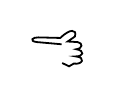
\begin{tikzpicture}[scale=.35]
\draw[line width=.65pt] (0,0) -- (-.9,.08) .. controls (-1.2,.12) and (-1.05,.26) .. (-.85,.25) -- (-.05,.23) .. controls (.3,.57) and (.57,.56) .. (.48,.28) -- (.22,.1) -- (.58,.08) .. controls (.78,.04) and (.77,-.15) .. (.53,-.18) .. controls (.86,-.23) and (.79,-.45) .. (.51,-.44) .. controls (.88,-.47) and (.77,-.75) .. (.44,-.7) -- (.27,-.8) -- (.02,-.68);
\end{tikzpicture}}}
L'inclusion $\supset$ est évidente du fait que les $X'^\circ$ sont $\subset X^\circ$. Prouvons $\subset$.
\deleted{Donc} Cela équivaut au
